\section{Experiments}
\suppressfloats[t]

\subsection{Evaluation validation}

The reported results come from a frozen evaluation snapshot included with the supplementary material. The snapshot contains raw run records, generated figures, the \hotpotmaxionbench{} manifest and checksums, and the conformance matrix. A strict-schema validation pass checked 72 run records and returned zero errors. Appendix Table~\ref{tab:portable-support} reports passing conformance and behavior-card coverage for FAISS CPU, LanceDB in-process, pgvector, and Qdrant; LanceDB service is excluded because it has no conformance row.

The supplementary material is intended to make each paper claim traceable. It contains the benchmark code, validation summary, conformance matrix, generated tables and figures, query-level paired-audit summaries, checksums, \hotpotmaxionbench{} Croissant-style metadata \citep{mlcommons2024croissant}, and a claim-evidence map. The main results below are tied to the recorded configs, conformance gate, objectives, and budget levels.

\subsection{Decision audit results}

We organize results around four deployment-audit questions. First, under the default 200 ms \maxrowp policy, FAISS CPU with bge-small is the policy-selected strict-latency configuration for all three workloads. Second, this decision is objective-sensitive: removing the p99 cap or optimizing quality changes selected configurations. Third, paired audits separate clear margins from aggregate near-ties. Fourth, budget stability is workload-dependent, so short screening runs cannot always replace B2 decisions.

\begin{figure}[t]
  \centering
  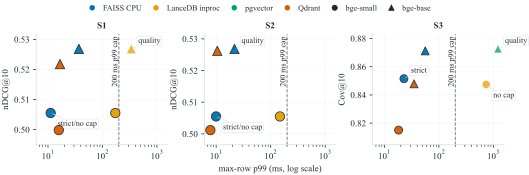
\includegraphics[width=\linewidth]{../figures/portable_decision_surface.pdf}
  \caption{Decision surface for the B2 audit. The strict 200 ms \maxrowp policy selects FAISS CPU/bge-small for S1 single-hop, S2 streaming, and S3 multi-evidence, but the no-p99 and quality-first markers show that the selection is conditional on objective and policy. Each panel uses a workload-specific zoomed y-axis.}
  \label{fig:decision-surface}
\end{figure}

\input{tables/neurips_main_results}

Table~\ref{tab:portable-main-results} is a strict-latency deployment-card summary. Under the 200 ms \maxrowp threshold, all three workloads select FAISS CPU with \texttt{BAAI/bge-small-en-v1.5}. The FAISS rows are exact FlatIP local-baseline rows, while the other rows include the configured store and adapter overheads; the table reports the decision under the recorded local runtime profile. The S1 single-hop selected row reaches \ndcg{} 0.506 with a 95\% confidence interval of 0.494--0.516 and \maxrowp 11.2 ms. S2 streaming selects the same engine and embedding, with \ndcg{} 0.506, \postinsertfive{} 0.830, and \maxrowp 10.0 ms. S3 multi-evidence selects FAISS CPU with \texttt{BAAI/bge-small-en-v1.5} at \ecov{} 0.852 and \maxrowp 22.8 ms.

S2 streaming measures agent-facing post-insert top-10 retrievability. S1 single-hop and the static-retrieval component of S2 streaming use the same 894-query BEIR-format evaluation pool under the 50K-document cap, which is why their static \ndcg{} and packed-token summaries can match. S2 streaming adds CRAG-500 write/retrieve probes after the adapter insert-plus-flush path returns. Across two B2 strict-choice repeats with 500 events each, 830 of 1{,}000 post-insert observations are retrieved by the 1s probe; no additional observations recover by 5s, leaving 170 of 1{,}000 absent at the 5s probe. Appendix Figure~\ref{fig:s2-postinsert}, Appendix Table~\ref{tab:s2-write-diagnostics}, and Appendix Table~\ref{tab:s2-post-insert-examples} report the fixed-probe diagnostics and example event/query/document IDs.

The benchmark-design ablation is reported in Appendix Table~\ref{tab:decision-error-ablation}. Its main implication is that removing any audit component changes the interpretation: the p99 gate separates strict-latency decisions from cost-only/no-p99 choices, objective separation prevents quality-first rows from being conflated with strict-latency rows, budget reporting exposes unstable S1 single-hop and S2 streaming screening runs, paired audits prevent aggregate near-ties from being overclaimed, and conformance filtering keeps unsupported service rows out of paper-facing tables.

\input{tables/portable_decision_table}

Table~\ref{tab:portable-decision-table} and Figure~\ref{fig:decision-surface} show objective sensitivity directly. The strict-latency and cost-only/no-p99 objectives agree for S1 single-hop and S2 streaming, but S3 multi-evidence shifts to LanceDB in-process with \texttt{BAAI/bge-small-en-v1.5} when the p99 cap is removed. Quality-first decisions differ more strongly: LanceDB in-process with \texttt{BAAI/bge-base-en-v1.5} leads S1 single-hop, FAISS CPU with \texttt{BAAI/bge-base-en-v1.5} leads S2 streaming, and the aggregate quality-first rule selects pgvector with \texttt{BAAI/bge-base-en-v1.5} for S3 multi-evidence. The threshold sweep makes the 200 ms policy explicit and auditable.

\begin{figure}[t]
  \centering
  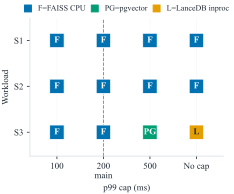
\includegraphics[width=0.62\linewidth]{../figures/portable_mvd_sensitivity.pdf}
  \caption{S3 multi-evidence is sensitive to relaxing the p99 policy, while S1 single-hop and S2 streaming keep the same policy-selected engine across the reported thresholds. This threshold sweep shows how MaxionBench reports decisions under stated local policies.}
  \label{fig:p99-sensitivity}
\end{figure}

\begin{figure}[t]
  \centering
  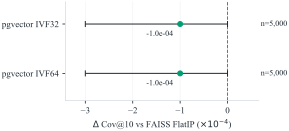
\includegraphics[width=0.72\linewidth]{../figures/s3_paired_audit_forest.pdf}
  \caption{Matched S3 multi-evidence paired audit. Against FAISS exact FlatIP on the same 5{,}000 bge-base queries, pgvector IVF32 and IVF64 have paired \ecov{} deltas whose 95\% intervals include zero, so the aggregate pgvector quality-first row shows no detectable advantage under matched queries.}
  \label{fig:s3-paired-audit}
\end{figure}

The S3 multi-evidence quality-first margin is the highest-risk aggregate claim, so we audit it with matched queries. Using all B2 rows, pgvector-base exceeds FAISS-base by only 0.00016 \ecov{} with an aggregate-row bootstrap interval of -0.00280 to 0.00304. The matched audit in Figure~\ref{fig:s3-paired-audit} removes even that apparent edge: pgvector IVF32 and IVF64 are each 0.0001 \ecov{} below FAISS exact FlatIP on the 5{,}000-query matched-audit subset, with paired intervals including zero. We therefore report no detectable pgvector advantage at this sample size rather than a quality win. Appendix Table~\ref{tab:s3-paired-quality} gives the numeric rows, and Appendix Table~\ref{tab:s3-all-evidence-hit} records the stricter binary all\_evidence\_hit@10 audit.

Appendix Table~\ref{tab:strict-decision-margins} makes the strict-latency decision margins explicit. For S1 single-hop and S2 streaming, FAISS CPU with \texttt{BAAI/bge-small-en-v1.5} matches the closest LanceDB in-process candidate on relevance quality and cost, so the deployment rule resolves the tie by lower \maxrowp and higher throughput. For S3 multi-evidence, Qdrant with \texttt{BAAI/bge-small-en-v1.5} is the nearest strict-cost alternative but is more expensive and lower quality, even though its \maxrowp is 4.6 ms lower in the repeat-aware table. The highest-quality strict-latency S3 multi-evidence option remains FAISS CPU with \texttt{BAAI/bge-base-en-v1.5}, which improves \ecov{} by 0.020 over \texttt{BAAI/bge-small-en-v1.5} but increases the normalized context-cost proxy by 0.704 and \maxrowp by 33.4 ms on the B2 audit rows.

The normalized context-cost proxy is stable under the coefficient sensitivity tested in the supplementary analysis. Appendix Table~\ref{tab:cost-sensitivity} rescales only \(c_{\mathrm{llm\_in}}\) from 0.1$\times$ to 10$\times$ and leaves all strict choices unchanged: S1 single-hop and S2 streaming have identical retrieved-token counts for the strict choice and nearest strict-cost competitor, while S3 multi-evidence FAISS/bge-small retrieves slightly fewer tokens than Qdrant/bge-small. Appendix Table~\ref{tab:latency-distribution} reports p50, p95, mean p99, and the min--max p99 range over B2 run rows for the recorded hardware/runtime profile.

\begin{figure}[t]
  \centering
  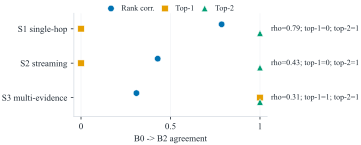
\includegraphics[width=0.62\linewidth]{../figures/portable_budget_stability.pdf}
  \caption{Budget stability is workload-dependent. B0 screening fails to preserve B2 top-1 choices for S1 single-hop and S2 streaming, while S3 multi-evidence preserves top-1 despite low full-rank Spearman correlation.}
  \label{fig:budget-effects}
\end{figure}

The budget analysis measures how much evidence is enough. B0-to-B2 top-1 agreement is zero for S1 single-hop and S2 streaming, with Spearman correlations 0.79 and 0.43, respectively. S3 multi-evidence has top-1 agreement of one but Spearman correlation 0.31, meaning that the selected strict-latency row is stable while lower-ranked alternatives remain noisy. The resulting decision card includes the budget level and stability statistics used to reach each recommendation.

\subsection{Targeted replication checks}

Targeted same-machine reruns support the decision-level conclusions and quantify tail-latency variation. Appendix Table~\ref{tab:strict-faiss-repeat-audit} shows that the strict FAISS CPU/bge-small choices reproduce the relevant quality values and remain under the 200 ms policy; the S3 multi-evidence bge-base rerun and Figure~\ref{fig:s3-paired-audit} support the objective-sensitivity story; and Appendix Table~\ref{tab:s2-competitor-check} reports a larger FAISS-versus-Qdrant S2 streaming paired check that finds no Qdrant quality or post-insert retrievability advantage. A final S3 local-scale check on the 66{,}635-document \hotpotmaxionbench{} corpus compares exact FAISS CPU and LanceDB in-process over the same 5{,}000-query cap: FAISS reports \ecov{} 0.8515 and p99 17.4 ms, while LanceDB reports \ecov{} 0.8514 and p99 172.4 ms; the existing validated Qdrant row reports \ecov{} 0.8117 and p99 21.0 ms. To isolate corpus-size effects, Appendix Table~\ref{tab:faiss-scale-stress} adds a controlled FAISS vector-scale stress check: at 1M vectors, exact FlatIP remains under 200 ms p99, but IVF reaches p99 9.45 ms with recall@10 0.9994 against FlatIP. Appendix Table~\ref{tab:cross-engine-scale-stress} adds a non-FAISS sanity check on the same vector construction: Qdrant HNSW reaches recall@10 0.9994 at 250K vectors with p99 8.91 ms and remains fully indexed at 1M vectors with recall@10 0.9994 and p99 10.05 ms. Read against the FAISS scale rows, the fully indexed Qdrant row shows that the local ordering can change by 250K vectors: FAISS exact is faster at 66K, while Qdrant HNSW is faster at 250K at near-exact recall. These checks support the local 50K--66K exact-baseline finding while showing why the paper does not present that ranking as production-scale evidence.
